%!TEX root = ../novoIndex.tex

Considerando a estratégia descrita na solução proposta, os resultados da execução das CNNs aplicadas ao problema de estimação de idade a partir de uma imagem de face são apresentados a seguir. Estes resultados estão organizados segundo abordagens sequenciais, que contemplam desde as técnicas mais elementares, e que vão aumentando o grau de complexidade conforme uso de estratégias específicas da prática de DL visando obter melhores resultados.

\section{Abordagem 1: LeNet e AlexNet com Imagens Normalizadas}%sem data augmentation, com normalização e sem equalização

	A primeira abordagem de treinamento considerou o uso dos modelos LeNet e AlexNet de maneira canônica, isto é, tais como são definidos na literatura. Adotou-se as funções de ativação não-lineares \emph{ReLU} e \emph{Leaky ReLU} por serem simples de calcular e por satisfazerem os critérios de continuidade e diferenciação, requeridos pelo algoritmo de \emph{backpropagation}, conforme discutido anteriormente na Seção \ref{subsec:modelos}.

	As imagens da base de dados foram normalizadas antes de serem apresentadas às redes, conforme a estratégia de pré-processamento previamente definida, isto é, todos os valores dos \emph{pixels} componentes das imagens foram escalonados para o intervalo $[0,1]$ por meio de uma divisão por $255$. Conforme mencionado, a prévia normalização das imagens antes da apresentação às CNNs colabora para uma melhor execução do gradiente descendente e diminui a variância nos pesos.

	Os treinamentos destas duas arquiteturas duraram aproximadamente $16$ e $12$ horas respectivamente, em uma instância do Google Compute Engine com 4 CPus virtuais e 15 GB de RAM. Os gráficos de treinamento e as retas zero obtidas a partir da apresentação do conjunto de teste aos modelos treinados podem ser vistos na Figura \ref{fig:lenet-abordagem1}.

	\begin{figure}[h!]
		\caption{Resultados do treinamento e teste da CNN LeNet de acordo com a Abordagem 1.}\label{fig:lenet-abordagem1}
	  \begin{subfigure}[hb]{0.5\linewidth}
	    \caption{RMSE de treinamento da arquitetura LeNet utilizando funções de ativação \emph{ReLU}.}

	    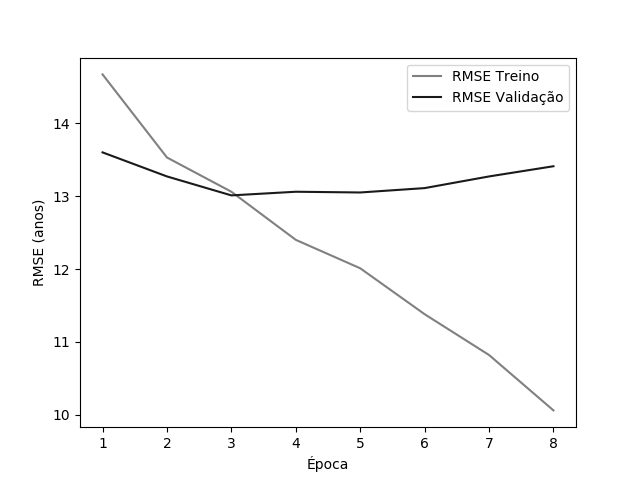
\includegraphics[width=\linewidth]{img/graficos/history/lenet/fig-history-image-treat-1-lenet-relu-rmse.png}%
	  \end{subfigure}%
		\begin{subfigure}[hb]{0.5\linewidth}
			\caption{Reta-0 LeNet \emph{ReLU}.}

			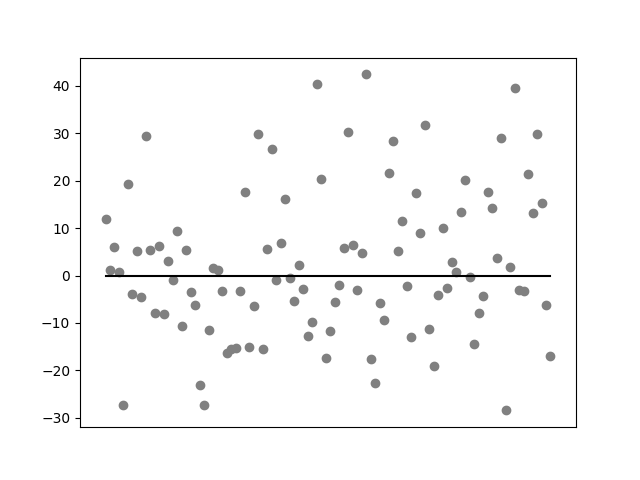
\includegraphics[width=\linewidth]{img/graficos/reta0/lenet/fig-reta-0-image-treat-1-lenet-relu.png}%
		\end{subfigure}\\
	  \begin{subfigure}[hb]{0.5\linewidth}
	    \caption{RMSE de treinamento da arquitetura LeNet utilizando funções de ativação \emph{Leaky ReLU}.}

	    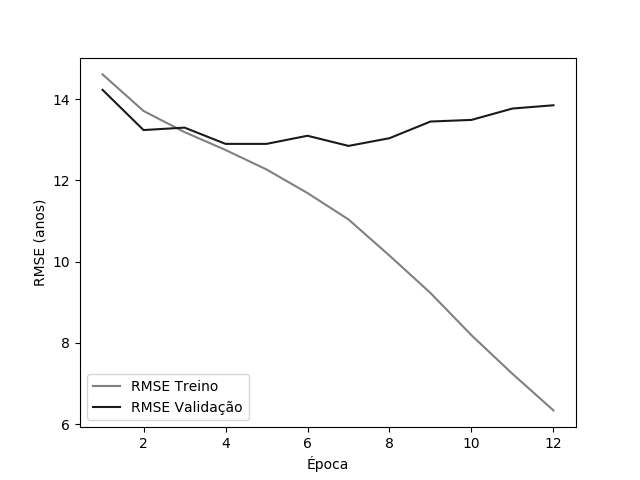
\includegraphics[width=\linewidth]{img/graficos/history/lenet/fig-history-image-treat-1-lenet-lrelu-rmse.png}
	  \end{subfigure}
		\begin{subfigure}[hb]{0.5\linewidth}
			\caption{Reta-0 LeNet \emph{Leaky ReLU}.}

		 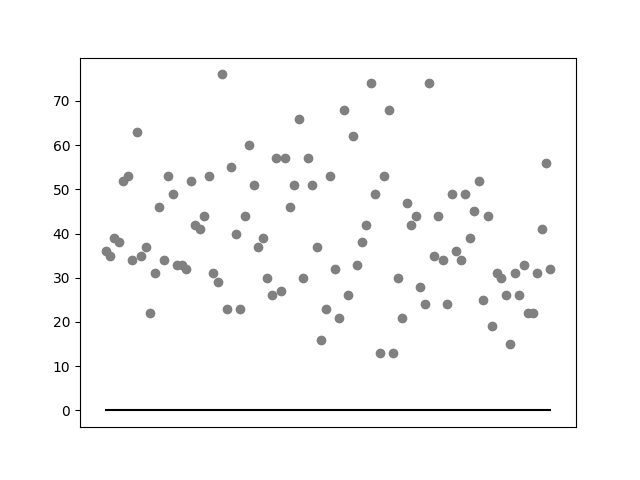
\includegraphics[width=\linewidth]{img/graficos/reta0/lenet/fig-reta-0-image-treat-1-lenet-lrelu.png}
		\end{subfigure}%
	\end{figure}

	\begin{figure}[ht!]
		\caption{Resultados do treinamento e teste da CNN AlexNet de acordo com a Abordagem 1.}\label{fig:alexnet-abordagem1}
		\begin{subfigure}[hb]{0.5\linewidth}
			\caption{Treinamento AlexNet \emph{ReLU}.}

			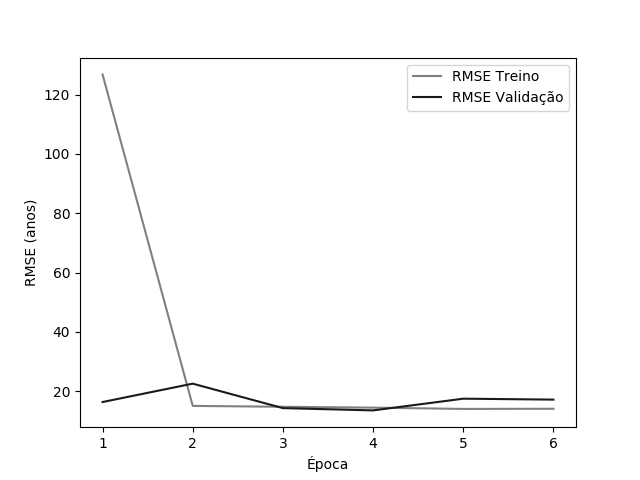
\includegraphics[width=\linewidth]{img/graficos/history/alexnet/fig-history-image-treat-1-alexnet-relu-rmse.png}
		\end{subfigure}
	  \begin{subfigure}[hb]{0.5\linewidth}
	    \caption{Reta-0 AlexNet \emph{ReLU}.}
	    \label{fig:reta0reludying}
	    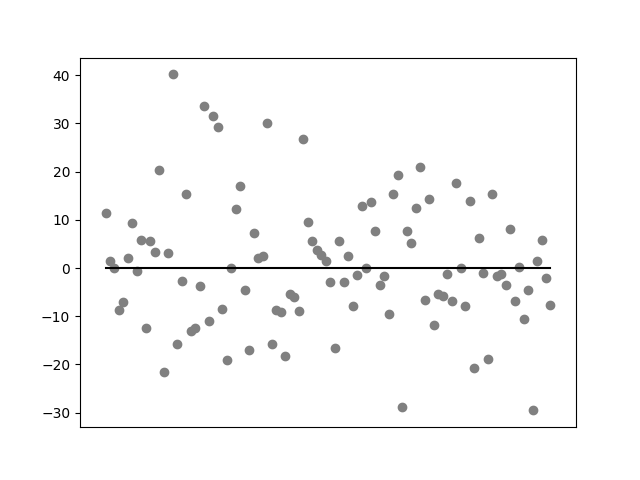
\includegraphics[width=\linewidth]{img/graficos/reta0/alexnet/fig-reta-0-image-treat-1-alexnet-relu.png}%
	  \end{subfigure}\\
		\begin{subfigure}[hb]{0.5\linewidth}
			\caption{Treinamento AlexNet \emph{Leaky ReLU}.}
			\label{fig:histalexlrelunorm}
	    \centering
			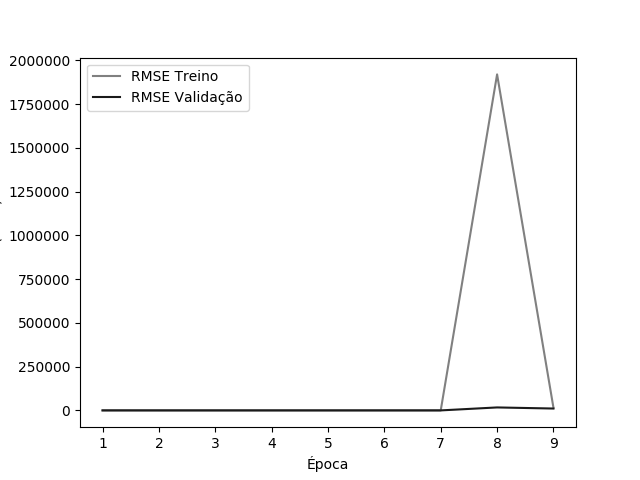
\includegraphics[width=\linewidth]{img/graficos/history/alexnet/fig-history-image-treat-1-alexnet-lrelu-rmse.png}
		\end{subfigure}
	  \begin{subfigure}[hb]{0.5\linewidth}
	    \caption{Reta-0 AlexNet \emph{Leaky ReLU}.}

	    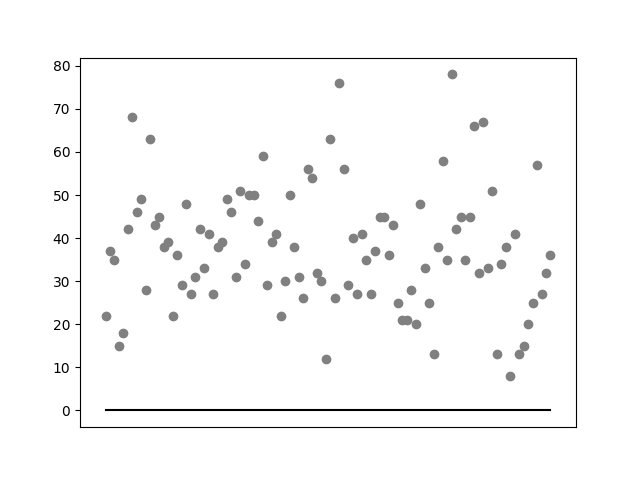
\includegraphics[width=\linewidth]{img/graficos/reta0/alexnet/fig-reta-0-image-treat-1-alexnet-lrelu.png}
	  \end{subfigure}%
	\end{figure}

	Obedecendo ao método de validação cruzada \emph{holdout} previamente mencionado, os resultados desta abordagem encontram-se sintetizados na Tabela \ref{tab:results-1}. De maneira geral, ambas as redes obtiveram melhor desempenho com o uso da função de ativação \emph{ReLU} em que, em particular,  a arquitetura LeNet apresento resultados ligeiramente superiores. Apesar disso, nota-se que o treinamento não seguiu de maneira estável, com grande variação entre as métricas de treinamento e validação, ocasionando \emph{early stopping} após um número relativamente curto de épocas. Tal cenário é sugestivo de \emph{overfitting}, especialmente mais evidentes nos casos em que se utilizou a função de ativação \emph{Leaky ReLU}.

  \begin{table}[!ht]
		\caption{Resultados do treino e teste dos modelos propostos na Abordagem 1.}
		\label{tab:results-1}
		\begin{center}
			\begin{tabular}{l l l l l}
				\toprule
				Rede & Função de ativação & Épocas & MAE Teste & RMSE Teste \\
				\midrule
				LeNet & \emph{ReLU}  & 4 & 10.53 & 13.55 \\
				LeNet & \emph{Leaky ReLU} & 8 & 38.33 & 40.82 \\
				AlexNet & \emph{ReLU}  & 5 & 11.03 & 13.76 \\
				AlexNet & \emph{Leaky ReLU} & 5 & 39.27 & 41.97 \\
				\bottomrule
			\end{tabular}
		\end{center}
	\end{table}

\section{Abordagem 2: Introduzindo \emph{Data Augmentation}}%com data augmentation, com normalização e sem equalização

	A abordagem anterior consistiu essencialmente da utilização dos modelos tal como foram definidos e com uma simples operação de adequação dos dados de entrada por meio de normalização. Porém, em problemas de Visão Computacional, é comum aplicar técnicas de \emph{data augmentation} com vistas a aumentar artificialmente o conjunto de dados, fazendo com que o modelo, em sua fase de treinamento, não seja exposto à mesma entrada em mais de uma ocasião. Esta estratégia de regularização colabora na mitigação do \emph{overfitting} e costuma promover uma melhor generalização \cite{chollet2017deep}.

	As técnicas de \emph{data augmentation} consideradas foram a rotação entre $0$ e $20$ graus no sentido horário ou anti-horário, zoom de $0.8$ a $1.2$ vezes, inversão horizontal com probabilidade de ocorrência de $0.5$ ou translação com probabilidade igual a $0.2$.

	Desta feita, após o aumento artificial do conjunto de dados, partiu-se então para o treinamento e teste dos modelos conforme a metodologia adotada, considerando as arquiteturas LeNet e AlexNet e as funções de ativação \emph{ReLU} e \emph{Leaky ReLU}. Os gráficos das métricas de desempenho coletadas durante o treinamento e a reta-0 obtida a partir dos dados de teste em cada uma destas quatro configurações são ilustrados nas Figuras \ref{fig:lenet-abordagem2} e \ref{fig:alexnet-abordagem2}.

	\begin{figure}[hb!]
		\caption{Resultados do treinamento e teste da CNN LeNet de acordo com a Abordagem 2.}\label{fig:lenet-abordagem2}
		\begin{subfigure}[hb]{0.5\linewidth}
			\caption{RMSE de treinamento da arquitetura LeNet utilizando funções de ativação \emph{ReLU}.}
			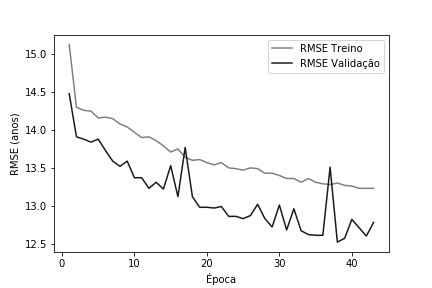
\includegraphics[width=\linewidth]{img/graficos/history/lenet/fig-history-image-treat-2-lenet-relu-rmse.png}%
		\end{subfigure}%
		\begin{subfigure}[hb]{0.5\linewidth}
			\caption{Reta-0 LeNet \emph{ReLU}.}
			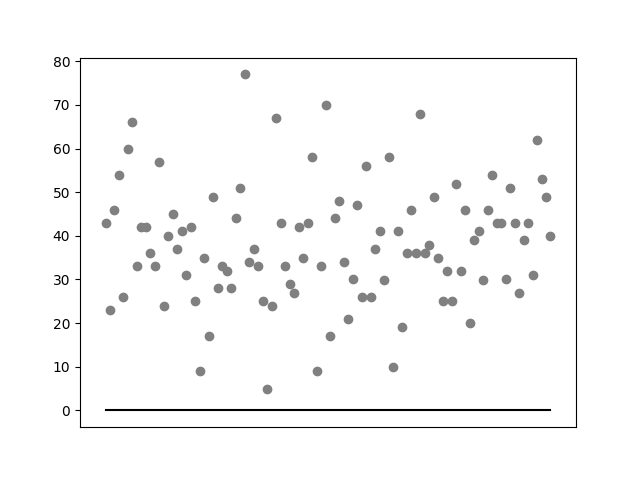
\includegraphics[width=\linewidth]{img/graficos/reta0/lenet/fig-reta-0-image-treat-2-lenet-relu.png}%
		\end{subfigure}\\
		\begin{subfigure}[hb]{0.5\linewidth}
			\caption{RMSE de treinamento da arquitetura LeNet utilizando funções de ativação \emph{Leaky ReLU}.}
			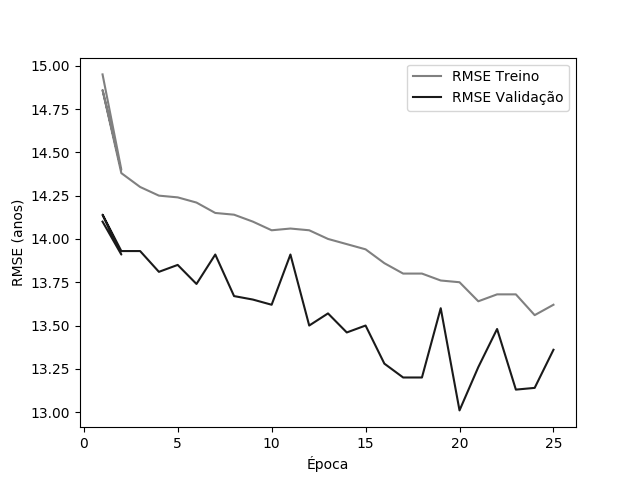
\includegraphics[width=\linewidth]{img/graficos/history/lenet/fig-history-image-treat-2-lenet-lrelu-rmse.png}
		\end{subfigure}
		\begin{subfigure}[hb]{0.5\linewidth}
			\caption{Reta-0 LeNet \emph{Leaky ReLU}.}
		 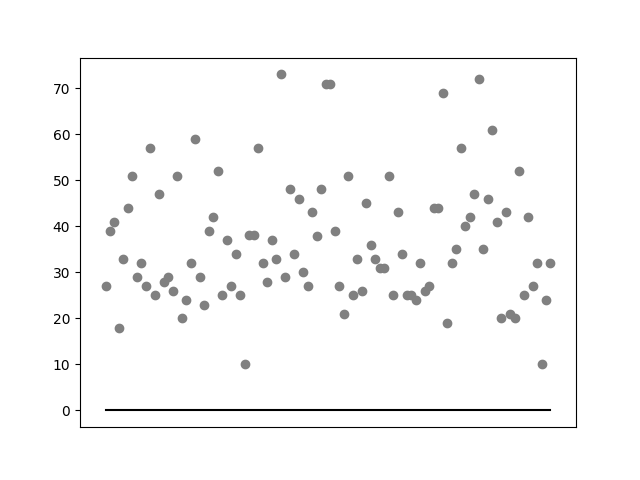
\includegraphics[width=\linewidth]{img/graficos/reta0/lenet/fig-reta-0-image-treat-2-lenet-lrelu.png}
		\end{subfigure}%
	\end{figure}

	\begin{figure}[ht!]
		\caption{Resultados do treinamento e teste da CNN AlexNet de acordo com a Abordagem 2.}\label{fig:alexnet-abordagem2}
		\begin{subfigure}[hb]{0.5\linewidth}
			\caption{Treinamento AlexNet \emph{ReLU}.}
			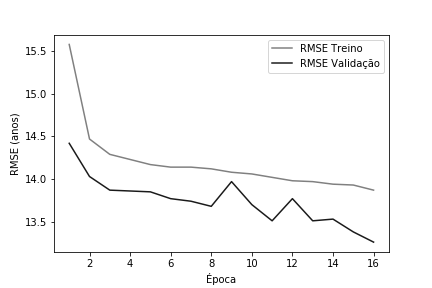
\includegraphics[width=\linewidth]{img/graficos/history/alexnet/fig-history-image-treat-2-alexnet-relu-rmse.png}
		\end{subfigure}
		\begin{subfigure}[hb]{0.5\linewidth}
			\caption{Reta-0 AlexNet \emph{ReLU}.}
			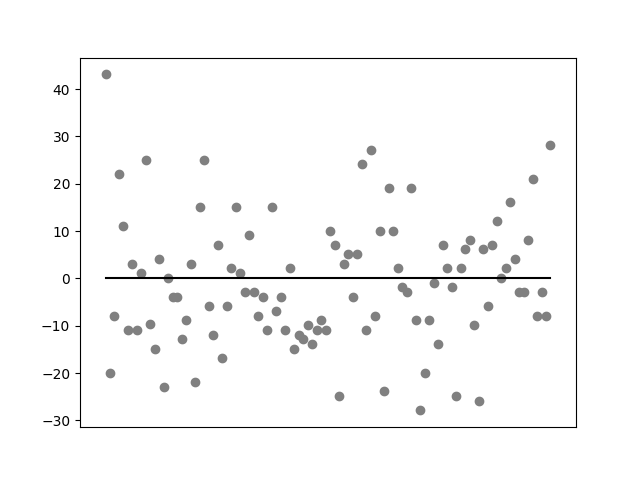
\includegraphics[width=\linewidth]{img/graficos/reta0/alexnet/fig-reta-0-image-treat-2-alexnet-relu.png}%
		\end{subfigure}\\
		\begin{subfigure}[hb]{0.5\linewidth}
			\caption{Treinamento AlexNet \emph{Leaky ReLU}.}
			\centering
			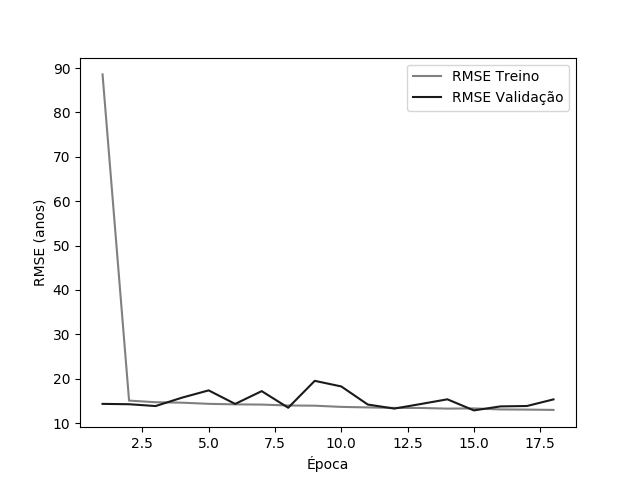
\includegraphics[width=\linewidth]{img/graficos/history/alexnet/fig-history-image-treat-2-alexnet-lrelu-rmse.png}
		\end{subfigure}
		\begin{subfigure}[hb]{0.5\linewidth}
			\caption{Reta-0 AlexNet \emph{Leaky ReLU}.}
			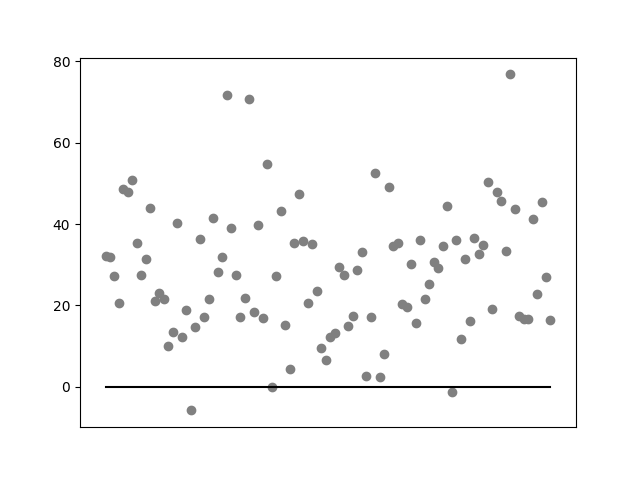
\includegraphics[width=\linewidth]{img/graficos/reta0/alexnet/fig-reta-0-image-treat-2-alexnet-lrelu.png}
		\end{subfigure}%
	\end{figure}

	De maneira análoga, as métricas de desempenho coletadas encontram-se detalhadas na Tabela \ref{tab:results2}. Nota-se que o número de épocas no treinamento foi maior que a abordagem anterior, indicando que houve um cenário mais favorável para o aprendizado dos padrões nos dados. De maneira geral, as métricas obtidas não fornecem uma evidência forte de que esta segunda abordagem produz resultados mais significativos que a primeira mas, no caso da CNN AlexNet com \emph{ReLU}, os resultados foram comparáveis. O efeito positivo esperado pelo \emph{data augmentation} não se mostrou tão evidente quanto se esperava inicialmente. Porém, isto pode acontecer em razão dos valores dos hiperparâmetros e da necessidade de melhor pré-processamento das imagens antes da apresentação às CNNs, o que motivou a realização da abordagem a seguir.

	\begin{table}[!hb]
		\caption{Resultados do treino e teste dos modelos propostos na Abordagem 2.}
		\label{tab:results2}
		\begin{center}
			\begin{tabular}{l l l l l}
				\toprule
				Rede & Função de ativação & Épocas & MAE Teste & RMSE Teste \\
				\midrule
				LeNet & \emph{ReLU}  & 39 & 37.85 & 40.27 \\
				LeNet & \emph{Leaky ReLU} & 21 & 38.50 & 41.06 \\
				AlexNet & \emph{ReLU}  & 16 & 11.59 & 14.59 \\
				AlexNet & \emph{Leaky ReLU} & 16 & 28.06 & 31.81 \\
				\bottomrule
			\end{tabular}
		\end{center}
	\end{table}



\section{Abordagem 3: Introduzindo Equalização de Histograma}%com data augmentation, com normalização e com equalização
	A terceira abordagem utilizou as imagens da base de dados normalizadas e técnicas de \emph{data augmentation} previamente mencionadas. Além disto, visando melhorar as métricas de desempenho, introduziu-se o processo de equalização das imagens por histograma, que ajusta o contraste da imagem utilizando o histograma de cores. Conforme mencionado na Seção \ref{subsec:limpeza}, este método aumenta o contraste global de imagens, especialmente quando os dados úteis da imagem são representados por cores próximas. No contexto da detecção de idade por meio da imagem da face de determinado indivíduo, a equalização por histograma reforça marcas de expressões e outras imperfeições \cite{acharya2005image}.

	Considerado uma nova equalização do conjunto de dados segundo o histograma, somado à normalização anterior e à aplicação de \emph{data augmentation}, consolidou-se então o treinamento e teste das redes LeNet e AlexNet com função de ativação \emph{ReLu} e \emph{Leaky ReLU} segundo a terceira abordagem. Os gráficos de treinamento e a reta-0 obtidos encontram-se nas Figuras \ref{fig:lenet-abordagem3} e \ref{fig:alexnet-abordagem3}, respectivamente. A partir destes gráficos, observa-se um treinamento mais consistente, com queda progressiva da perda à medida que se avançam as épocas. Apesar disso, nota-se também que houve retrocessos na métrica de perda da validação ao longo do treinamento, o que promoveu \emph{early stopping}.


	\begin{figure}[hb!]
		\caption{Resultados do treinamento e teste da CNN LeNet de acordo com a Abordagem 3.}\label{fig:lenet-abordagem3}
		\begin{subfigure}[hb]{0.5\linewidth}
			\caption{RMSE de treinamento da arquitetura LeNet utilizando funções de ativação \emph{ReLU}.}
			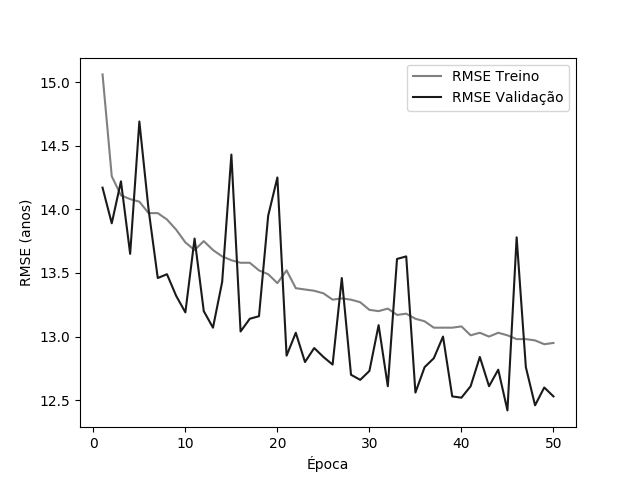
\includegraphics[width=\linewidth]{img/graficos/history/lenet/fig-history-image-treat-3-lenet-relu-rmse.png}%
		\end{subfigure}%
		\begin{subfigure}[hb]{0.5\linewidth}
			\caption{Reta-0 LeNet \emph{ReLU}.}
			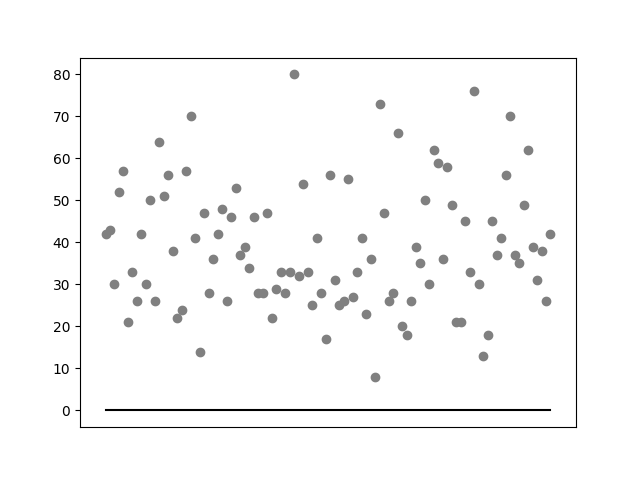
\includegraphics[width=\linewidth]{img/graficos/reta0/lenet/fig-reta-0-image-treat-3-lenet-relu.png}%
		\end{subfigure}\\
		\begin{subfigure}[hb]{0.5\linewidth}
			\caption{RMSE de treinamento da arquitetura LeNet utilizando funções de ativação \emph{Leaky ReLU}.}
			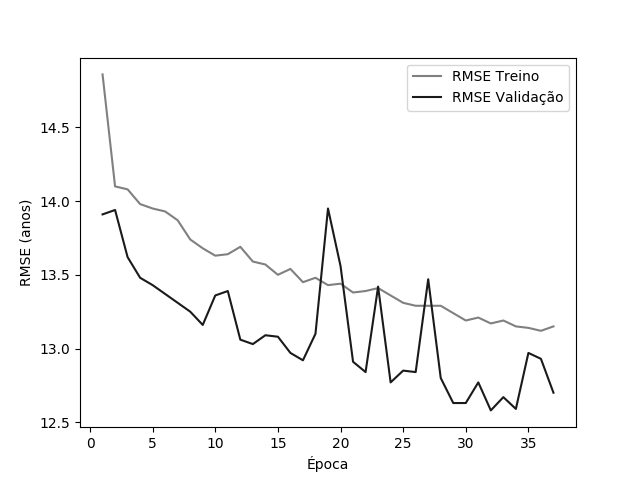
\includegraphics[width=\linewidth]{img/graficos/history/lenet/fig-history-image-treat-3-lenet-lrelu-rmse.png}
		\end{subfigure}
		\begin{subfigure}[hb]{0.5\linewidth}
			\caption{Reta-0 LeNet \emph{Leaky ReLU}.}
		 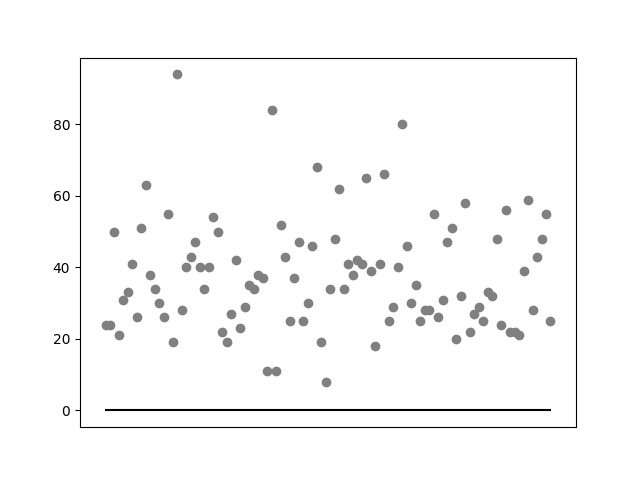
\includegraphics[width=\linewidth]{img/graficos/reta0/lenet/fig-reta-0-image-treat-3-lenet-lrelu.png}
		\end{subfigure}%
	\end{figure}

	\begin{figure}[hb!]
		\caption{Resultados do treinamento e teste da CNN AlexNet de acordo com a Abordagem 3.}\label{fig:alexnet-abordagem3}
		\begin{subfigure}[hb]{0.5\linewidth}
			\caption{RMSE de treinamento da arquitetura AlexNet utilizando funções de ativação \emph{ReLU}.}
			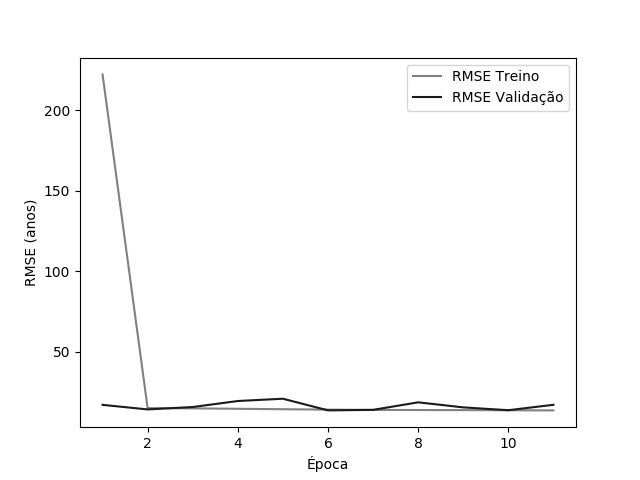
\includegraphics[width=\linewidth]{img/graficos/history/alexnet/fig-history-image-treat-3-alexnet-relu-rmse.png}
		\end{subfigure}
		\begin{subfigure}[hb]{0.5\linewidth}
			\caption{Reta-0 AlexNet \emph{ReLU}.}
			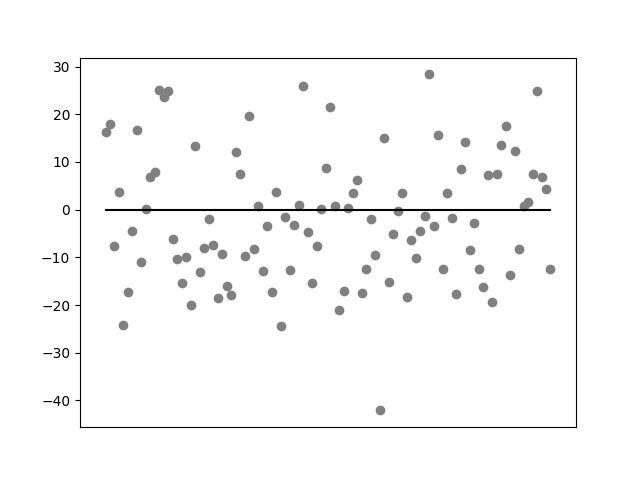
\includegraphics[width=\linewidth]{img/graficos/reta0/alexnet/fig-reta-0-image-treat-3-alexnet-relu.png}%
		\end{subfigure}\\
		\begin{subfigure}[hb]{0.5\linewidth}
			\caption{RMSE de treinamento da arquitetura AlexNet utilizando funções de ativação RMSE de treinamento da arquitetura LeNet utilizando funções de ativação \emph{Leaky ReLU}.}
			\centering
			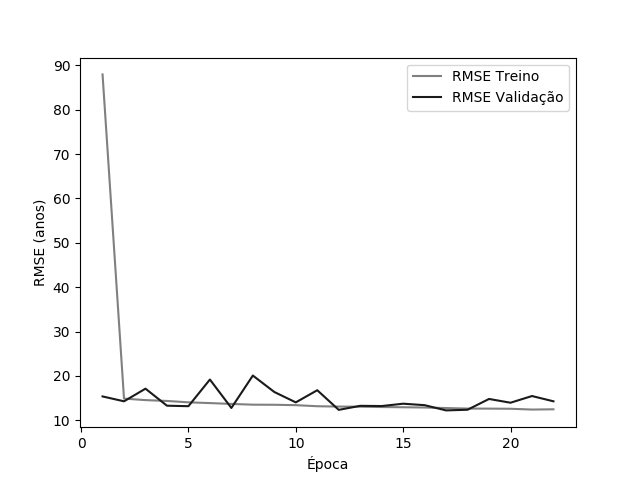
\includegraphics[width=\linewidth]{img/graficos/history/alexnet/fig-history-image-treat-3-alexnet-lrelu-rmse.png}
		\end{subfigure}
		\begin{subfigure}[hb]{0.5\linewidth}
			\caption{Reta-0 AlexNet \emph{Leaky ReLU}.}
			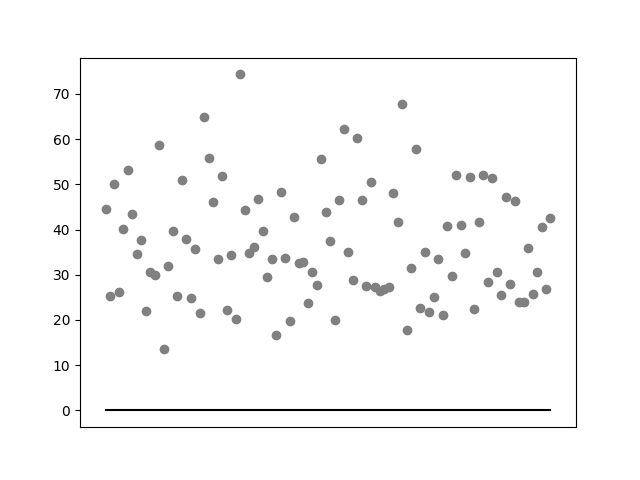
\includegraphics[width=\linewidth]{img/graficos/reta0/alexnet/fig-reta-0-image-treat-3-alexnet-lrelu.png}
		\end{subfigure}%
	\end{figure}

	Obedecendo ao método de validação cruzada \emph{holdout} previamente mencionado, os resultados desta abordagem encontram-se sintetizados na Tabela \ref{tab:results-3}. É interessante notar que o aumento nas épocas do treinamento não foi efetivo em obter melhores métricas de testes. Tem-se que, embora as CNNs aprendam por mais épocas que nos cenários anteriores, este aprendizado é menor para fins de generalização. Apesar de estar havendo um esforço de pré-processamento por meio de \emph{data augmentation} e de equalização por histograma, seguindo práticas tipicamente adotadas em trabalhos desta área \cite{chollet2017deep}, as melhorias promovidas por estas estratégias são de cunho heurístico, podendo ser boas em determinados cenários, mas não garantidamente em todos, tal como ocorreu no contexto em questão.

	\begin{table}[!ht]
		\caption{Resultados do treino e teste dos modelos propostos na Abordagem 3.}
		\label{tab:results-3}
		\centering
		\begin{tabular}{l l l l l l l}
				\toprule
				Rede & Função de ativação & Épocas & MAE Teste & RMSE Teste \\
				\midrule
				LeNet & \emph{ReLU} & 46 &  38.66 & 41.20 \\
				LeNet & \emph{Leaky ReLU} &  38 & 38.26 & 40.85 \\
				AlexNet & \emph{ReLU} & 7 & 13.10 & 15.88 \\
				AlexNet & \emph{Leaky ReLU} & 18 & 35.25 & 38.04 \\
				\bottomrule
			\end{tabular}
	\end{table}

\section{Abordagem 4: Utilizando MAE para o Cálculo da Perda}%com data augmentation, com normalização e com equalização, usando mae pra loss
	A análise dos gráficos de treinamento das redes anteriores levou à suposição de que a métrica utilizada para a atualização dos pesos RMSE estivesse trazendo instabilidade para o treinamento. Desta maneira, esta abordagem considera a rede com melhor desempenho verificado até então, a LeNet com função de ativação \emph{ReLU}, imagens normalizadas mas sem \emph{data augmentation} ou equalização por histograma descrita ainda na Abordagem 1. Porém, decidiu-se sujeitar as entradas desta rede às técnicas de \emph{data augmentation} e equalização por histograma, mas com a utilização do MAE para cálculo da perda.

	Esta abordagem foi considerada em virtude do treinamento com o otimizador \emph{Adam} construir superfícies estocásticas de erro a partir da métrica de perda. Assim, após treinamento e teste, obteve-se os gráficos ilustrados  nas Figuras \ref{fig:lenet-abordagem4}.

	\begin{figure}[hb!]
		\caption{Resultados do treinamento e teste da CNN LeNet de acordo com a Abordagem 4.}\label{fig:lenet-abordagem4}
		\begin{subfigure}[hb]{0.5\linewidth}
			\caption{MAE de treinamento da arquitetura LeNet utilizando funções de ativação \emph{ReLU}.}
			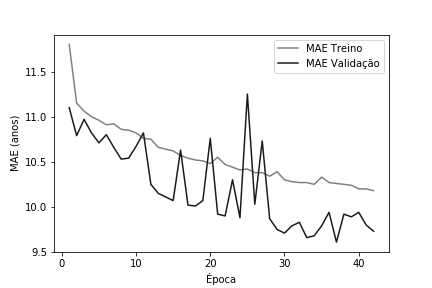
\includegraphics[width=\linewidth]{img/graficos/history/lenet/fig-history-abordagem-4-lenet-relu-mae.png}%
		\end{subfigure}%
		\begin{subfigure}[hb]{0.5\linewidth}
			\caption{Reta-0 LeNet \emph{ReLU}.}
			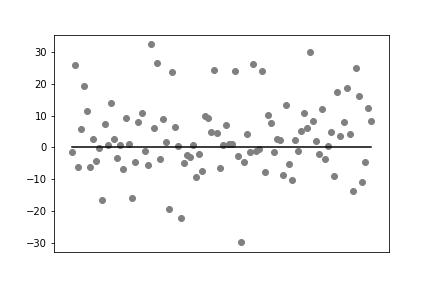
\includegraphics[width=\linewidth]{img/graficos/reta0/lenet/fig-reta-0-abordagem-4-lenet-relu.png}%
		\end{subfigure}
	\end{figure}

	Obedecendo ao método de validação cruzada \emph{holdout} previamente mencionado, os resultados desta abordagem encontram-se sintetizados na Tabela \ref{tab:results-4}.

	\begin{table}[!ht]
		\centering
		\caption{Resultados do treino e teste do modelo proposto na Abordagem 4.}
		\label{tab:results-4}
			\begin{tabular}{l l l l l l l}
				\toprule
				Rede & Função de ativação & Épocas & MAE Teste & RMSE Teste \\
				\midrule
				LeNet & \emph{Leaky ReLU} & 38 & 9.98 & 12.91 \\
				\bottomrule
			\end{tabular}
	\end{table}

	Os resultados obtidos evidenciam melhores métricas de desempenho até então, oferecendo diretrizes positivas a cerca das estratégias adotadas. Apesar da identificação de uma rede satisfatória até então, fica o questionamento se as melhorias obtidas em si foram introduzidas pelas heurísticas de pré-processamento ou se são intrínsecas do modelo adotado. Como a equalização por histograma e os processos de \emph{data augmentation} introduzem ônus de pré-processamento aos dados, desejou-se verificar se o desempenho positivo desta rede seria mantido mesmo sem tais práticas, o que motivou a realização da abordagem seguinte.

\section{Abordagem 5: LeNet Apenas com Normalização da Entrada}% sem data augmentation, com normalização e sem equalização, usando mae pra loss, batch de 128, sem patience
	A quinta abordagem também adotou a rede com melhor desempenho obtido até o momento, a LeNet descrita na Abordagme 1, com função de ativação \emph{ReLU}, treinada apenas com imagens da base de dados normalizadas, mas sem equalização de histograma nem tampouco técnicas de \emph{data augmentation}. Seguiu-se utilizando a métrica MAE para o cálculo da perda e da atualização dos pesos. Buscando garantir maior estabilidade nas métricas de desempenho durante o treinamento, aumentou-se o tamanho do batch para $128$, com vistas a estimar melhor a superfície de erro à medida que o algoritmo de otimização percorre o gradiente descendente.

	\begin{figure}[hb!]
		\caption{Resultados do treinamento e teste da CNN LeNet de acordo com a Abordagem 5.}\label{fig:lenet-abordagem5}
		\begin{subfigure}[hb]{0.5\linewidth}
			\caption{MAE de treinamento da arquitetura LeNet utilizando funções de ativação \emph{ReLU}.}
			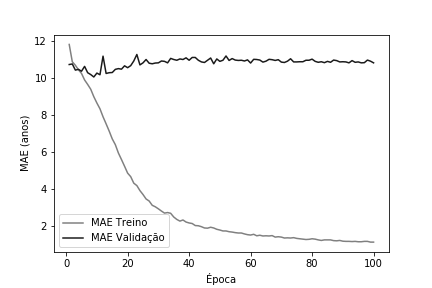
\includegraphics[width=\linewidth]{img/graficos/history/lenet/fig-history-abordagem-5-lenet-relu-mae.png}%
		\end{subfigure}%
		\begin{subfigure}[hb]{0.5\linewidth}
			\caption{Reta-0 LeNet \emph{ReLU}.}
			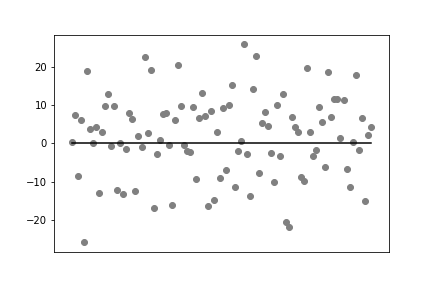
\includegraphics[width=\linewidth]{img/graficos/reta0/lenet/fig-reta-0-abordagem-5-lenet-relu.png}%
		\end{subfigure}\\
	\end{figure}

	Obedecendo ao método de validação cruzada \emph{holdout}, os resultados desta abordagem encontram-se sintetizados na Tabela \ref{tab:results-5}. É interessante notar que não houve melhorias na métrica de desempenho, pelo contrário, o erro aumentou em relação ao cenário anterior, sugerindo que as práticas de pré-processamento colaboram positivamente no melhor aprendizado das características da tarefa considerada. Uma vez que foram exploradas diferentes práticas de treinamento das redes LeNet e AlexNet, em que as melhorias alcançadas estagnaram após a quarta abordagem, partiu-se então para a avaliação de arquiteturas mais profundas aplicadas ao problema considerado, o que ensejou as abordagens a seguir.

	\begin{table}[!ht]
		\centering
		\caption{Resultados do treino e teste dos modelos propostos na Abordagem 5.}
		\label{tab:results-5}
			\begin{tabular}{l l l l l l l}
				\toprule
				Rede & Função de ativação & Épocas & MAE Teste & RMSE Teste \\
				\midrule
				LeNet & \emph{ReLU} & 9 &  10.09 & 13.04 \\
				\bottomrule
			\end{tabular}
		\end{table}


\section{Abordagem 6: VGG-16 e Dados Normalizados}
	A sexta abordagem considerou a utilização da arquitetura VGG-16, previamente apresentada na Seção \ref{subsec:modelos}. Para utilização neste contexto, de maneira análoga aos cenários anteriores, removeu-se a camada de saída, tipicamente utilizada para fins de classificação, e adicionou-se uma camada densa com função de ativação \emph{ReLU}. Embora tipicamente esta rede seja utilizada com \emph{transfer learning} do conjunto de dados ImageNet, optou-se por seguir a prática adotada nas demais redes, com inicialização aleatória dos pesos e treinamento integral com o conjunto de dados apenas sujeito à normalização.

	Em decorrência do treinamento e teste nos mesmos moldes dos cenários anteriores, obteve-se os gráficos ilustrados na Figura \ref{fig:vgg-abordagem6}. As métricas de desempenho obtidas são elencadas na Tabela \ref{tab:results-6}.

		\begin{figure}[hb!]
			\caption{Resultados do treinamento e teste da CNN VGG-16 de acordo com a Abordagem 6.}\label{fig:vgg-abordagem6}
			\begin{subfigure}[hb]{0.5\linewidth}
				\caption{MAE de treinamento da arquitetura VGG-16 utilizando funções de ativação \emph{ReLU}.}
				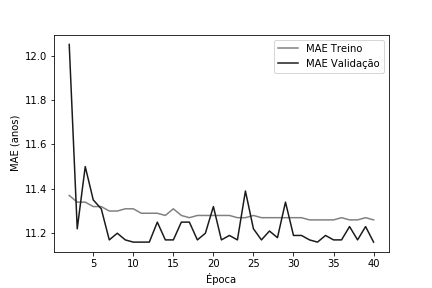
\includegraphics[width=\linewidth]{img/graficos/history/vgg16/fig-history-abordagem6-vgg16-relu-mae.png}%
			\end{subfigure}%
			\begin{subfigure}[hb]{0.5\linewidth}
				\caption{Reta-0 VGG-16 \emph{ReLU}.}
				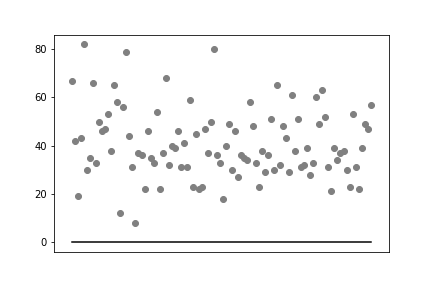
\includegraphics[width=\linewidth]{img/graficos/reta0/vgg16/fig-reta-0-abordagem6-vgg16-relu.png}%
			\end{subfigure}\\
		\end{figure}

		\begin{table}[!ht]
			\centering
			\caption{Resultados do treino e teste dos modelos propostos na Abordagem 6.}
			\label{tab:results-6}
			\begin{tabular}{l l l l l l l}
				\toprule
				Rede & Função de ativação & Épocas & MAE Teste & RMSE Teste \\
				\midrule
				VGG-16 & \emph{ReLU} & 11 & 40.90 & 38.35 \\
				\bottomrule
			\end{tabular}
		\end{table}

		É interessante notar que a rede VGG-16 é mais profunda em termos de camadas que as redes LeNet e AlexNet, o que impacta em uma maior quantidade de parâmetros livres a serem calculados e que acaba por exigir mais recursos computacionais para seu treino. Segundo as ideias de DL, imagina-se que uma rede com um número maior de camadas hierárquicas seja capaz de produzir melhores representações, impactando positivamente no aprendizado da tarefa. Apesar disso, teve desempenho aquém. Uma suposição para este resultado é que a rede sofreu \emph{dying ReLU problem}, pois apenas produziu saídas iguais a $37.05$ para todas as imagens dadas como entrada, maximizando o erro aferido no teste. Para contornar este problema, esta arquitetura foi novamente testada, mas introduzindo também \emph{data augmentation} e normalização por equalização de histograma.



\section{Abordagem 7: VGG-16 com \emph{Data Augmentation} e Equalização de Histograma}

	A rede VGG-16 utilizada nesta abordagem foi instanciada e treinada com os mesmos parâmetros descritos na Abordagem 6, porém, passou-se a utilizar \emph{data augmentation} e equalização de histograma, obedecendo às mesmas práticas de configuração utilizada nas Abordagens 2 a 4 para as redes LeNet e AlexNet e dos resultados positivos observados.

	Os resultados obtidos do treinamento e teste encontram-se ilustrados nos gráficos do treinamento e reta-0 da Figura \ref{fig:vgg-abordagem7} e detalhados na Tabela \ref{tab:results-7}. É interessante notar que as técnicas para mitigar \emph{overfitting} não foram efetivas para contornar o \emph{dying ReLU problem} previamente verificado, impactando em métricas análogas de erro.

		\begin{figure}[h!]
			\caption{Resultados do treinamento e teste da CNN VGG-16 de acordo com a Abordagem 7.}\label{fig:vgg-abordagem7}
			\begin{subfigure}[hb]{0.5\linewidth}
				\caption{MAE de treinamento da arquitetura VGG-16 utilizando funções de ativação \emph{ReLU}.}
				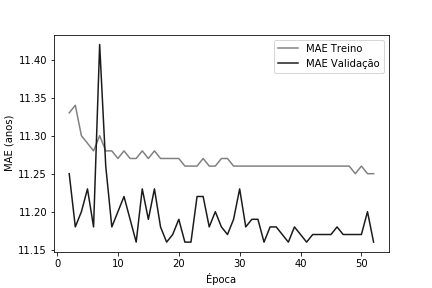
\includegraphics[width=\linewidth]{img/graficos/history/vgg16/fig-history-abordagem7-vgg16-relu-mae.png}%
			\end{subfigure}%
			\begin{subfigure}[hb]{0.5\linewidth}
				\caption{Reta-0 VGG-16 \emph{ReLU}.}
				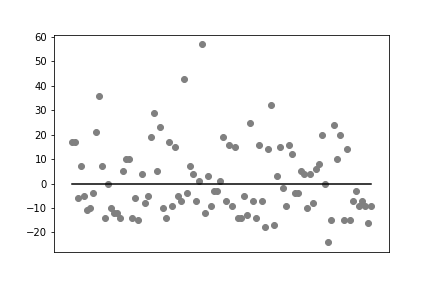
\includegraphics[width=\linewidth]{img/graficos/reta0/vgg16/fig-reta-0-abordagem7-vgg16-relu.png}%
			\end{subfigure}\\
		\end{figure}

\begin{table}[!ht]
	\centering
	\caption{Resultados do treino e teste dos modelos propostos na Abordagem 7.}
	\label{tab:results-7}
		\begin{tabular}{l l l l l }
			\toprule
			Rede & Função de ativação & Épocas & MAE Teste & RMSE Teste \\
			\midrule
			VGG-16 & \emph{ReLU} & 23 & 40.99 & 38.39 \\
			\bottomrule
		\end{tabular}
	\end{table}

	A partir da análise dos resultados obtidos, observa-se a VGG-16 também sofreu dificuldades durante o treinamento. Esta rede possivelmente foi vítima de \emph{dying ReLU problem}, mesmo havendo mudanças nas entradas apresentadas, haja vista que o modelo obtido testado após o treino seguindo a abordagem descrita previa apenas o valor $37.02$ para todas as imagens de entrada apresentadas. Portanto, optou-se por realizar ajustes diretamente nos parâmetros da rede, conforme é descrito na próxima solução para treinamento considerada.

\section{Abordagem 8: VGG-16 com \emph{data augmentation}, \emph{Transfer Learning} e \emph{Leaky ReLU}}

 A abordagem agora considerada tenta endereçar de maneira mais objetiva a superação do \emph{dying ReLU problem}, pois considera a adoção da função de ativação \emph{Leaky ReLU} que não está sujeita à este fenômeno, segundo a literatura \cite{djork2015elus}. Além disto, tentou-se utilizar uma taxa de aprendizado inicial maior, igual a $0.003$, tentando favorecer uma caminhada mais objetiva no gradiente descendente em função do método de otimização utilizado. É importante salientar que, embora possa implicar em mais avanços que impliquem na eventual convergência, esta taxa de aprendizado torna o treinamento consideravelmente mais instável. \emph{Data augmentation} e equalização de histograma foram empregados seguindo os mesmos objetivo e configuração descritos em estratégias anteriores. \emph{Transfer Learning} de pesos obtidos a partir do treinamento da VGG-16 para classificação de objetos por meio da base de dados ImageNet foi empregado com o objetivo de inicializar os pesos de maneira a facilitar a convergência do modelo.

 O comportamento do MAE durante o treinamento e a reta-0 obtida durante o teste da VGG-16 obtida utilizando estas configurações podem ser visualizados na Figura \ref{fig:vgg-abordagem8}. Na Tabela \ref{tab:results-8} estão as métricas de desempenho RMSE e MAE.

 \begin{figure}[h!]
	 \caption{Resultados do treinamento e teste da CNN VGG-16 de acordo com a Abordagem 8.}\label{fig:vgg-abordagem8}
	 \begin{subfigure}[hb]{0.5\linewidth}
		 \caption{MAE de treinamento da arquitetura VGG-16 utilizando funções de ativação \emph{Leaky ReLU}.}
		 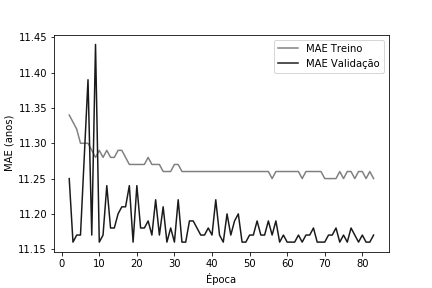
\includegraphics[width=\linewidth]{img/graficos/history/vgg16/fig-history-abordagem9-vgg16-lrelu-mae.png}%
	 \end{subfigure}%
	 \begin{subfigure}[hb]{0.5\linewidth}
		 \caption{Reta-0 VGG-16 \emph{Leaky ReLU}.}
		 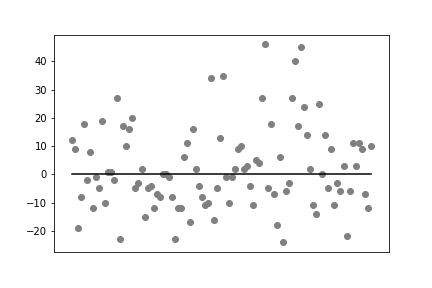
\includegraphics[width=\linewidth]{img/graficos/reta0/vgg16/fig-reta-0-abordagem9-vgg16-lrelu.png}%
	 \end{subfigure}\\
 \end{figure}

\begin{table}[!ht]
\centering
\caption{Resultados do treino e teste dos modelos propostos na Abordagem 8.}
\label{tab:results-8}
 \begin{tabular}{l l l l l }
	 \toprule
	 Rede & Função de ativação & Épocas & MAE Teste & RMSE Teste \\
	 \midrule
	 VGG-16 & \emph{Leaky ReLU} & 83 & 11.02 & 14.24 \\
	 \bottomrule
 \end{tabular}
\end{table}

Assim como as VGG-16 treinadas anteriormente, esta CNN prevê um valor fixo para qualquer entrada apresentada, neste caso $36.99$. Este é um indicador de que o modelo continua sofrendo \emph{dying ReLU problem}, apesar da configuração descrita nesta abordagem. Salienta-se que existem diversas estratégias, descritas na literatura, capazes de contornar este problema. Porém, dada a característica empírica e o tempo de treinamento das CNNs, em especial modelos extensos como a VGG-16, optou-se por buscar um modelo de CNN tido como mais simples.

\section{Abordagem 9: SqueezeNet}

	A última abordagem considerada neste trabalho, buscando sempre a perspectiva de melhores métricas e uma boa adequação ao contexto final de utilização do modelo, tratou do treinamento e teste da rede SqueezeNet. Dada a proposição recente deste modelo na literatura, ainda há poucos guias práticos sobre sugestões de uso e inicialização. Assim, esta arquitetura foi mantida tal como inicialmente proposta, mas considerou-se o uso de \emph{data augmentation} e equalização de histograma, objetivando os mesmos ganhos verificados nas abordagens anteriores melhor sucedidas até então.

	Os resultados obtidos pelo treinamento e teste encontram-se ilustrados nos gráficos do treinamento e reta-0 da Figura \ref{fig:squeeze-abordagem9} e detalhados na Tabela \ref{tab:results-9}.

	\begin{figure}[h!]
		\caption{Resultados do treinamento e teste da CNN SqueezeNet de acordo com a Abordagem 9.}\label{fig:squeeze-abordagem9}
		\begin{subfigure}[hb]{0.5\linewidth}
			\caption{MAE de treinamento da arquitetura SqueezeNet utilizando função de ativação \emph{ReLU} e \emph{data augmentation}.}
			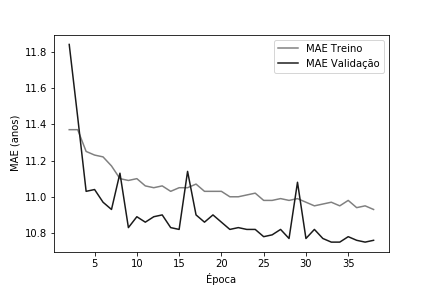
\includegraphics[width=\linewidth]{img/graficos/history/squeeze/fig-history-abordagem-squeeze1-squeeze-relu-mae.png}%
		\end{subfigure}%
		\begin{subfigure}[hb]{0.5\linewidth}
			\caption{Reta-0 SqueezeNet.}
			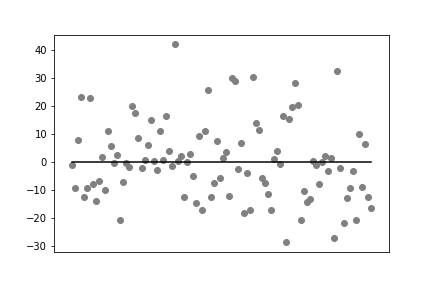
\includegraphics[width=\linewidth]{img/graficos/reta0/squeeze/fig-reta-0-abordagem-squeeze1-squeeze-relu.png}%
		\end{subfigure}\\
	\end{figure}

	\begin{table}[!ht]
	\centering
	\caption{Resultado do teste da SqueezeNet proposta na Abordagem 9.}
	\label{tab:results-9}
		\begin{tabular}{l l l l l }
			\toprule
			Rede & Função de ativação & Épocas & MAE Teste & RMSE Teste \\
			\midrule
			SqueezeNet & \emph{ReLU} & 38 & 10.72 & 13.84 \\
			\bottomrule
		\end{tabular}
	\end{table}

	A SqueezeNet obteve métricas de desempenho satisfatórias considerando os valores obtidos por outras redes treinadas utilizando diferentes abordagens. Esta CNN foi capaz de gerar valores diferenciados para cada imagem de entrada, ou seja, não caiu em \emph{dying ReLU problem} mesmo empregando \emph{ReLU} como função de ativação para suas camadas. Estes resultados são expressivos ao se considerar os recursos necessários para executar um sistema de tempo real utilizanod uma CNN, já que a SqueezeNet ocupa menos de 1 MB de memória \cite{squeezenet} e obteve, para este problema, resultados similares aos de redes que necessitam de mais espeço e poder de processamento, a citar LeNet e AlexNet.

\section{Sumarizando os Resultados}

Considerando todas as abordagens conduzidas, a Tabela \ref{tab:resultsAll} sintetiza todos os treinamentos e testes realizados e os resultados obtidos da métrica de desempenho MAE adotada para esta tarefa. Pode-se identificar então que, para a tarefa elencada, a rede com melhor desempenho observado foi a LeNet descrita na Abordagem 4, que se utiliza de funções de ativação \emph{ReLU}, com imagens de entrada sujeitas às técnicas de \emph{data augmentation} e equalização por histograma. Esta abordagem também trouxe a mudança de métrica utilizada para o cálculo da perda e da atualização dos pesos durante o treinamento de RMSE para MAE, o que acabou trazendo mais estabilidade para o treinamento das redes.

\begin{table}[b]
	\caption{Sumário dos resultados obtidos de todas as abordagens conduzidas.}
	\label{tab:resultsAll}
  \begin{center}
	\resizebox{0.68\linewidth}{!} {
		\begin{tabular}{cccccc}
			\toprule
			Abordagem & Rede & Função de ativação & Épocas & MAE Teste & RMSE Teste \\
			\midrule
			1 & LeNet & \emph{ReLU}  & 4 & 10.53 & 13.55 \\
			1 & LeNet & \emph{Leaky ReLU} & 8 & 38.33 & 40.82 \\
			1 & AlexNet & \emph{ReLU}  & 5 & 11.03 & 13.76 \\
			1 & AlexNet & \emph{Leaky ReLU} & 5 & 39.27 & 41.97 \\
			2 & LeNet & \emph{ReLU}  & 39 & 37.85 & 40.27 \\
			2 & LeNet & \emph{Leaky ReLU} & 21 & 38.50 & 41.06 \\
			2 & AlexNet & \emph{ReLU}  & 16 & 11.59 & 14.59 \\
			2 & AlexNet & \emph{Leaky ReLU} & 16 & 28.06 & 31.81 \\
			3 & LeNet & \emph{ReLU} & 46 &  38.66 & 41.20 \\
			3 & LeNet & \emph{Leaky ReLU} &  38 & 38.26 & 40.85 \\
			3 & AlexNet & \emph{ReLU} & 7 & 13.10 & 15.88 \\
			3 & AlexNet & \emph{Leaky ReLU} & 18 & 35.25 & 38.04 \\
			4 &	LeNet & \emph{Leaky ReLU} & 38 & 9.98 & 12.91 \\
			5 & LeNet & \emph{ReLU} & 9 &  10.09 & 13.04 \\
			6 & VGG-16 & \emph{ReLU} & 11 & 40.90 & 38.35 \\
			7 & VGG-16 & \emph{ReLU} & 23 & 40.99 & 38.39 \\
			8 & VGG-16 & \emph{Leaky ReLU} & 83 & 11.02 & 14.24 \\
			9 & SqueezeNet & \emph{ReLU} & 38 & 10.72 & 13.84 \\
			\bottomrule
		\end{tabular}
		}
  \end{center}
\end{table}


É interessante notar que o ajuste de parâmetros e hiperparâmetros para as redes neurais convolucionais segue as mesmas dificuldades das redes neurais \emph{multilayer perceptron}, em que a superfície de erro é hiperdimensional e complexa, e que, quanto maior o número de pesos na rede, maior é o espaço de busca pelos parâmetros ideais, dificultando, por conseguinte, a tarefa de encontrá-los \cite{Teresa:Livro}. No caso das CNNs, em especial, soma-se isto ao fato do aprendizado destas redes ser naturalmente mais oneroso em virtude do número de operações necessárias para realização das convoluções e do algoritmo de \emph{backpropagation}.
